\documentclass{article}

% -------------- PACOTE GERAL -------------- %
\usepackage{helper}

% -------------- CONFIGURACOES DA BIBLIOGRAFIA -------------- %
\addbibresource{bib.bib}

% -------------- TITULO E INFORMACOES -------------- %
\title{N-Body Initial Values Conditioner}
\author{potalej}
\date{August 2026}

% -------------- DOCUMENTO -------------- %
\begin{document}
\maketitle

\tableofcontents

% -------------- SECTIONS -------------- %
\section{Introduction}

In the N-body problem we don't have the solution explicitly in general, so we need to approximate it numerically and therefore we need to choose initial conditions that we want to simulate. In many cases we may think in astrophysics terms, using density profiles like Plummer, Hernquist \textit{etc}. But sometimes we may need just specific things from the problem, like having some values for the first integrals or start in (virial) equilibrium.

This package do this: given state vectors $\vet m \in \R^N$, $\vet q \in \R^{3N}$ and $\vet p \in \R^{3N}$, it applies a conditioner that moves the vectors to state vectors that correspond to what we want, like having the total energy $E = 0$, as long as it's physically possible.

For now, we can condition the state vectors to have the desired first integrals and to start in equilibrium.


\section{Some concepts}
In the N-body problem (in 3d) we have 10 first integrals, being:
\begin{itemize}
    \item The total energy $E$;
    \item The total angular momentum $\vet J \in \R^3$;
    \item The total linear momentum $\vet P \in \R^3$;
    \item The ``center of mass'' $\vet G \in \R^3$.
\end{itemize}

The quotation marks is due to $\vet G$ not being the actual center of mass, but a kind of reference frame:
\begin{equation}
    \vet G = M \vet q_{com} - t \vet P,
    \quad
    M = \sum_{a=1}^N m_a.
\end{equation}

A good thing about the N-body problem is that it's potential is invariant under translations, so we ever start with $\vet q_{com} = \vet 0$ without any loss of generality. The translation that we need to do with some state vectors to obtain $\vet q_{com} = \vet 0$ is
\begin{equation}
    \vet q_a^{\text{new}} = \vet q_a - \vet q_{com}, \ a = 1, 2, ..., N.
\end{equation}
It's evident that any homothety over the new positions doesn't affect the new c.o.m., so this is made only one time at the begin of every method.

Another observation we need to do is that the classic potential energy
\begin{equation}
V = - \sum_{b < a} G \dfrac{m_a m_b}{\norma{\vet q_b - \vet q_a}}
= - \sum_{b < a} G \dfrac{m_a m_b}{r_{ab}}
\end{equation}
is \textbf{homogeneous} with degree $-1$. However, when we consider the softened problem, the softened potential energy isn't homogeneous anymore:
\begin{equation}
V_\varepsilon = - \sum_{b < a} G \dfrac{m_a m_b}{\sqrt{r_{ab}^2 + \varepsilon^2}}.
\end{equation}


\section{An iterative method to condition the first integrals}
A first attempt may be to condition all the first integrals separately. 

\subsection{Total linear momentum}
Starting by the total linear momentum $\vet P$, we can apply the same idea of the c.o.m., but we need to choose a weight vector $\vet w \in \R^N$ and find some vector $\vet W_P$ such that
\begin{equation}
    \sum_{a=1}^N \vet p_a + w_a \vet W_P = 
    \vet P + \vet W_P = \tilde{\vet P}
    \Rightarrow
    \vet W_P = \tilde{\vet P} - \vet P,
\end{equation}
where $\tilde{\vet P}$ is the desired total linear momentum and we have
\begin{equation}\label{eq:total_linear_momentum_conditioner_iterative}
\vet p_a^{\text{new}} = \vet p_a + w_a (\tilde{\vet P} - \vet P).
\end{equation}
The simplest choose may be $w_a = m_a / M$.

\subsection{Total angular momentum}
For the total angular momentum $\vet J$, the thing is a little more complicated. Although we developed it independetly, Aarseth already used the idea in a two-body problem \cite[p. 135]{aarseth_gravitational_2003}.

Consider a particle with position $\vet r$ and a vector $\vet \omega$ that defines a rotation axis from which distante to $\vet r$ is $\rho$ and forms an angle $\xi$. Consider that the velocitiy of the particle wrt the axis $\vet \omega$ is $\vet v$ (see figure \ref{fig:angular_3d}).

\begin{figure}[H]
    \centering
    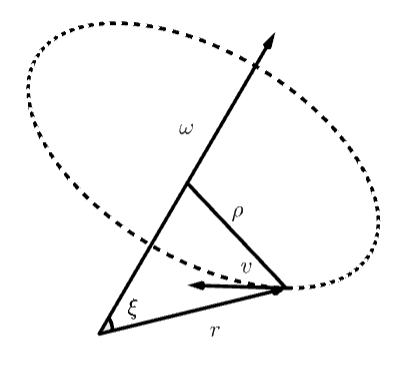
\includegraphics[width=0.3\linewidth]{img/rotation.png}
    \caption{Representation of a particle and a rotation axis.}
    \label{fig:angular_3d}
\end{figure}

In this situation, we have that $\norma{\vet v} = \rho \norma{\vet \omega}$ and $\sin \xi = \rho / \norma{\vet r}$. Because $\vet v \perp \vet \omega$ and $\vet v \perp \vet r$, we can conclude that $\vet v \parallel (\vet r \times \vet \omega)$. More than this,
\begin{equation}
\norma{\vet r \times \vet \omega} = \norma{\vet r} \norma{\vet \omega} \sin \xi = \norma{\vet v}
\ \therefore \ \vet v = \vet r \times \vet \omega.
\end{equation}

The angular momentum $\vet J$ is perpendicular to $\vet r$ and $\vet v$ too, but $\vet J$ and $\vet \omega$ are collinear only when $\vet r \perp \vet \omega$. However, we can construct an operator $\bm W: \R^3 \to \R^3$ that takes $\vet \omega$ to $\vet J$:
\begin{equation}
\bm W = m \begin{bmatrix}
- (r_2^2 + r_3^2) & r_1 r_2 & r_1 r_3 \\
r_1 r_2 & - (r_1^2 + r_3^2) & r_2 r_3 \\
r_1 r_3 & r_2 r_3 & - (r_1^2 + r_2^2)
\end{bmatrix}.
\end{equation}
This operator is called the \textbf{inertia tensor} (although is not really a \textit{tensor}), and in the literature it appears with the opposite sign sometimes. We can write the angular momentum with:
\begin{equation}
\vet J = \bm W \vet \omega.
\end{equation}

With more than one particle, we can define a common rotation axis $\vet \omega$ and from it apply transformations over the angular velocity of each body. Let $\bm W_T = \sum_{a=1}^N \vet W_a$. To obtain the desired $\tilde{\vet J}$, we need to find the $\vet \omega$ such that
\begin{equation}\label{eq:J_conditioner_system}
\bm W_T \vet \omega = \tilde{\vet J} - \vet J
\end{equation}
and apply the transformation
\begin{equation}\label{eq:total_angular_momentum_conditioner_iterative}
\vet p_a^{\text{new}} = \vet p_a + m_a \vet q_a \times \vet \omega.
\end{equation}

\subsection{Classic total energy}
In the classic total energy we have the homogeneous potential, so we can just look for $\alpha$ and $\beta$ and define $\vet q^{\text{new}} = \alpha^{-1} \vet q$ and $\vet p^{\text{new}} = \beta \vet p_a$ such that
\begin{equation}
    T(\beta \vet p) + V(\alpha^{-1} \vet q)
    = \beta^2 T + \alpha V = \tilde E.
\end{equation}
We have many forms to solve this equation. If $\tilde E \geq 0$, we can just set $\alpha = 1$ and obtain
\begin{equation}
\beta = \pm \sqrt{\dfrac{\tilde E - V}{T}}.
\end{equation}
In other cases, we can just choose
\begin{equation}
    \alpha = 1 + \dfrac{\tilde E}{V},
    \quad
    \beta = \sqrt{- \dfrac{V}{T}}.
\end{equation}

\subsection{Softened total energy}
In the softened case, if the desired total energy is greater than zero the process is the same, as long we don't need to change the positions. If $E < 0$, we can apply the same factor over the velocities:
\begin{equation}
\beta = \sqrt{- \dfrac{V}{T}},
\end{equation}
and it gives a kinect energy $\tilde T = \beta^2 T(\vet p)$. What we need to obtain $\tilde E$ is a factor $\alpha$ such that $V_{\varepsilon}(\alpha^{-1} \vet q) + \tilde T = \tilde E$. Being $\alpha = 1/\varepsilon \mu$, we have
\begin{equation}
\varepsilon^{-1} V_1 (\mu \vet q) + \tilde T - \tilde E = 0.
\end{equation}
Let $f(\mu)$ the left side. The problem is to find a root $\mu$ for this equation, and it can be done by the Newton-Raphson method, given
\begin{equation}
    f'(\mu) = \varepsilon^{-1} \sum_{b < a}^N \dfrac{G m_a m_b r_{ab}^2}{(r_{ab}^2 \mu^2 + 1)^{3/2}}.
\end{equation}

\subsection{The algorithm}
It's evident that the applications impact each other. What we can do is define the application $A_{iter} = \iota_E \circ \iota_J \circ \iota_P$ and suppose that this have a fixed point, so we can apply it some times and get a small error in the final result.

The algorithm is then:
\begin{enumerate}
    \item Move the c.o.m. to the origin;
    \item Apply the total linear momentum conditioner \eqref{eq:total_linear_momentum_conditioner_iterative}.
    \item Apply the total angular momentum conditioner \eqref{eq:total_angular_momentum_conditioner_iterative}.
    \item Apply one of the total energy conditioners.
    \item If the error on the first integrals isn't acceptable, go back to 2. 
\end{enumerate}

%%%%%%%%%%%%%%%%%%%%%%%%%%%%%%%%%%%%%%%
\section{A direct method to condition the first integrals without softening}
In the homogeneous case (without softening), we can incorporate all the conditioners into one direct conditioner, i.e., it doesn't need iterations and have machine precision. Observe that, as everywhere, we consider the c.o.m. at origin.

To conditionate the momenta constants we can just unify the two methods, considering the weights the normalized masses:
\begin{equation}
\vet p_a^{\text{new}} = \vet p_a - \dfrac{m_a}{M} (\vet P - \tilde{\vet P}) - m_a \vet q_a \times \vet \omega,
\quad
\bm W_T \vet \omega = \vet J - \tilde{\vet J}.
\end{equation}
% It's easy to see that we get what we want:
% \begin{equation}
% \sum_{a=1}^N \vet p_a^{\text{new}} = \vet P - \vet P + \tilde{\vet P} - M \vet q_{com} \times \vet \omega = \tilde{\vet P}.
% \end{equation}
% \begin{align}
% \sum_{a=1}^N \vet q_a \times \vet p_a^{\text{new}}
% &= \vet J - \left(\sum_{a=1}^N \dfrac{m_a}{M} \vet q_a\right) \times (\vet P - \tilde{\vet P}) - \sum_{a=1}^N m_a \vet q_a \times (\vet q_a \times \vet \omega) \nonumber
% = \vet J - \bm W_T \vet \omega = \tilde{\vet J}.
% \end{align}

For the energy, we also use homothety, but because applying $\vet p \mapsto \beta \vet p$ affects the momenta constants and $\vet q \mapsto \alpha^{-1} \vet q$ affects the angular momentum, we need to include these constants:
\begin{equation}
\vet p_a^{\text{\new}} = \beta \left(\vet p_a - \dfrac{m_a}{M} \left(\vet P - \dfrac{1}{\beta} \tilde{\vet P}\right) - m_a \vet q_a \times \vet \omega\right),
\quad
\bm W_T \vet \omega = \vet J - \dfrac{\alpha}{\beta} \tilde{\vet J}.
\end{equation}

Fixing $\alpha$, we have
\begin{equation}
    \beta = \pm \sqrt{- \dfrac{V + S_2}{S_1}},
\end{equation}
where
\begin{equation}
S_1 = T - \dfrac{1}{2 M} \norma{\vet P}^2 + \dfrac{1}{2} \prodint{\vet \omega_0}{\vet J^0},
\quad
\bm W_T \vet \omega_0 = \vet J,
\end{equation}
\begin{equation}
S_2 = \dfrac{1}{2} \norma{\tilde{\vet P}}^2 - \dfrac{\alpha^2}{2} \prodint{\tilde{\vet \omega}}{\tilde{\vet J}},
\quad
\bm W_T \tilde{\vet \omega} = \tilde{\vet J}.
\end{equation}

The process to obtain this simplification is in the Appendix \ref{appendix:simplifying}.

%%%%%%%%%%%%%%%%%5
\section{Starting in equilibrium}
To stardarize the numerical study of the N-body problem, Heggie proposed some default values \cite{heggie_mathieu_unidades}:
\begin{equation}
E = - 1/4, \quad R_V = 1, \quad G = 1, \quad M = 1,
\end{equation}
where $R_V \approx - GM^2/(2 V)$ is called the \textbf{virial radius}. The word \textit{virial} is related to the equilibrium that occurs when the second derivative of the moment of inertia
\begin{equation}
I = \sum_{a=1}^N m_a \norma{\vet q_a}^2 = -\dfrac{1}{2} \operatorname{Tr}{\bm W_T},
\end{equation}
that is given by the Lagrange-Jacobi identity:
\begin{equation}\label{eq:lagrange-jacobi-expanded}
\ddot I = 4 E - 2 \sum_{a=1}^N \prodint{\vet q_a}{\derpar{V}{\vet q_a}},
\end{equation}
that can be simplified in the case of homogeneous potential by the Euler's theorem for homogeneous functions:
\begin{equation}
\ddot I = 4 E - 2 V.
\end{equation}

To construct initial conditions with these default values, we apply the same process to condition the first integrals, normalize the masses and apply a one more conditioner: letting $Q_v = \sqrt{- V/{2T}}$, we take $\beta = V/(2E) = -2V$ and apply:
\begin{equation}
    \vet q^{\text{new}} = \beta \vet q,
    \quad
    \vet p^{\text{new}} = \dfrac{Q_V}{\sqrt{\beta}} \vet p.
\end{equation}

\subsection{Softened potential for negative energies}
With the loss of homogeneity, we need to use the equation \eqref{eq:lagrange-jacobi-expanded}, and we can do something related to what we did for the iterative method: we apply (using $V_\varepsilon$)
\begin{equation}
    \vet p^{\text{new}} = \dfrac{Q_V}{\sqrt{\beta}} \vet p.
\end{equation}
To conditionate the virial radius we need to have
\begin{equation}
    T(\vet p^{\text{new}}) = \tilde E - V_\varepsilon(\alpha^{-1} \vet q).
\end{equation}
We can define the following function $f$:
\begin{align}
f(\alpha) 
&= 2 \tilde E - V_\varepsilon(\alpha^{-1}V) + \sum_{a=1}^N \prodint{\vet F_a^{(\varepsilon)}(\alpha^{-1} \vet q)}{\alpha^{-1}\vet q_a} \nonumber \\
&= 2 \tilde E - 2 \alpha V_{\varepsilon \alpha}(\vet q) + \alpha^2 \sum_{a=1}^N \prodint{\vet F_a^{(\alpha \varepsilon)}(\vet q)}{\vet q_a}.
\end{align}

Again, we need to use an iterative method to evaluate $\alpha$, like the Newton-Raphson method. For this, being $\mu = \alpha^{-1}$ we get:
\begin{equation}
f'(\mu^{-1}) = 2 \mu^{-2} V_{\varepsilon / \mu}(\vet q) - \dfrac{2}{\mu} \der{V_{\varepsilon/\mu}}{\mu} - \dfrac{1}{\mu^2} \sum_{a=1}^N \prodint{\vet F_a^{(\varepsilon/\mu)}(\vet q)}{\vet q_a} + \dfrac{1}{\mu} \sum_{a=1} \prodint{\der{F_a^{(\varepsilon/\mu)}(\vet q)}{\mu}}{\vet q_a}.
\end{equation}

The derivative of forces wrt $\mu$ are
\begin{equation}
\der{\vet F_a^{(\varepsilon/\mu)}(\vet q)}{\mu}
= \dfrac{3 \varepsilon^2}{\mu^3} \sum_{b \neq a} G m_a m_b \dfrac{\vet q_b - \vet q_a}{(r_{ab}^2 + (\varepsilon/\mu)^2)^{5/2}},
\end{equation}
and of the potential is
\begin{equation}
    \der{V_{\varepsilon/\mu}}{\mu} = - \dfrac{\varepsilon^2 G}{\mu^3} \sum_{a < b} \dfrac{m_a m_b}{(r_{ab}^2 + (\varepsilon/\mu)^2)^{3/2}}.
\end{equation}

As the initial candidate we can take $\mu_0 = - 2 V_{\varepsilon}(\vet q)$, that is the solution for the classical problem. At the end, we have a potential that with the desired $\tilde E$ guarantee equilibrium. The kinect energy is not the desired, so we re-conditionate the velocities:
\begin{equation}
    \tilde p = \left(\dfrac{V(\alpha^{-1} \vet q)}{\tilde E} - 1\right)^{1/2} \vet p.
\end{equation}


\appendix
\section{Simplifying the direct method}\label{appendix:simplifying}
Fixing $\alpha$, we get
\begin{equation}
    \beta = \sqrt{- \dfrac{V}{T(\vet p^{\text{new}}/\beta)}}.
\end{equation}

Expanding:
\begin{align}
    T(\vet p^{\text new}/\beta) 
    &= \sum_{a=1}^N \dfrac{1}{2 m_a} \norma{\vet p_a - \dfrac{m_a}{M} \left(\vet P - \dfrac{1}{\beta} \tilde{\vet P}\right) - m_a \vet q_a \times \vet \omega}^2 \nonumber \\
    &= \sum_{a=1}^N \dfrac{1}{2 m_a} \norma{\left(\vet p_a - \dfrac{m_a}{M} \vet P - m_a \vet q_a \times \bm W_T^{-1} \vet J\right) + \dfrac{1}{\beta} \left(\dfrac{m_a}{M} \tilde{\vet P} + \alpha m_a \vet q_a \times \bm W_T^{-1} \tilde{\vet J}\right)}^2 \nonumber \\
    &= \sum_{a=1}^N \dfrac{1}{2 m_a} \left(\norma{\vet K_a^1}^2 + \dfrac{1}{\beta^2} \norma{\vet K_a^2}^2 + \dfrac{2}{\beta} \prodint{\vet K_a^1}{\vet K_a^2}\right).
\end{align}

Although it looks more complicated, we can simplify it a lot. First,
\begin{equation}
    \sum_{a=1}^N \dfrac{1}{2m_a} \prodint{\vet K_a^1}{\vet K_a^2} = 0.
\end{equation}

Now, being $\vet u, \vet v \in \R^3$, it's vector product can be write in a matrix form:
\begin{equation}
    \vet u \times \vet v = [\vet u]_{\times} \vet v,
    \quad
    [\vet u]_\times = \begin{bmatrix}
        0 & - u_3 & u_2 \\ u_3 & 0 & -u_1 \\ -u_2 & u_1 & 0
    \end{bmatrix}.
\end{equation}
This matrix has the following property:
\begin{equation}
    [\vet u]_\times^T [\vet u]_\times = \norma{\vet u}^2 \bm {Id}_3 - \vet u \vet u^T,
\end{equation}
so we can write
\begin{equation}
\norma{\vet u \times \vet v}^2 = \vet v^T (\norma{|vet u}^2 \bm{Id}_3 - \vet u \vet u^T) \vet v.
\end{equation}

Therefore we can write the inertia tensor for a body as
\begin{equation}
\bm W_a = m_a (\vet q_a \vet q_a^T - \norma{\vet q_a}^2 \bm{Id}_3),
\end{equation}
and
\begin{equation}
\sum_{a=1}^N \norma{\vet q_a \times \bm W_T^{-1} \vet J}^2
= - \vet J^T \bm W_T^{-T} \bm W_T \bm W_T^{-1} \vet J
= - \vet J^T \bm W_T^{-1} \vet J.
\end{equation}

The simplification in trivial from here.


% -------------- Bibliograhy -------------- %
\printbibliography

\end{document}